
\chapter{Project Structure and Requirements}

This chapter describes the structure of the project. First the overall organization and then the individual components are explained. Following that, the prerequisites and processes for building and/or running the code used in various parts of the project are briefly described.

\section{Requirements}
\label{SECTION:REQS}
This project requires a Linux system with {\itshape gcc}, {\itshape bash}, and a recent version of Python 3 with the {\itshape numpy} package to run the benchmarks. Additional Python packages are required to view and execute the analysis notebooks. {\itshape Jupyter Notebook}, {\itshape matplotlib},  {\itshape pandas}, and {\itshape seaborne} can be installed using the python package installer {\itshape pip}. The Jupyter Notebook requires at least Python 3.3.

\section{Directory Structure}
Figure \ref{FIG:folders} shows the file structure of the project.  First of all, the documentation (i.e.  this pdf) is in the \texttt{docs} folder, and the latex source files are in \texttt{latex}. The \texttt{ann\_1.2.2} directory contains the neighbor search C++ libraries that is examined. The \texttt{nanoflann} directory is an additional neighbor search library.  The folders \texttt{src} and \texttt{bin} contain the C++ source files (described in Section \ref{SECTION:SRC}) and their compiled binaries, respectively.  The \texttt{scripts} directory is home to the test case generation scripts (described in Section \ref{SECTION:TESTCASESCRIPTS}) and test execution scripts (see Chapter \ref{CHAPTER:BENCHMARKING}).  The \texttt{test} directory contains the working directories of the test runs and the result data.   Finally, the folder \texttt{analysis} contains the Jupyter iPython notebooks that were used in the examination and analysis of the results.  These are described in more detail in Section \ref{SECTION:NOTEBOOKS}.

\begin{figure}[h]
	\centering
	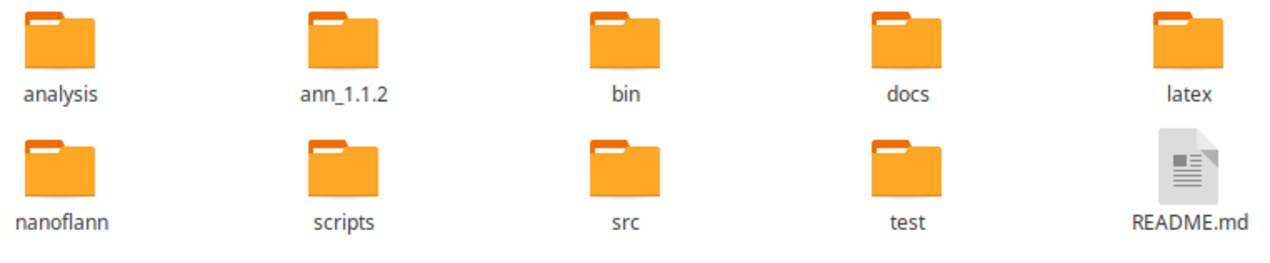
\includegraphics[width=0.75\textwidth]{figures/project_folders.pdf}
	\caption{The root-level structure of the project repository.}
      \label{FIG:folders}
\end{figure}

\section{Search Methods}
\label{SECTION:SRC}

The nearest neighbor search methods are implemented in C++. The \texttt{src} directory contains the source files. The linked-cell method is implemented in \texttt{fr\_cellLinkedList.cpp}. For the ANN method, there are multiple variants. First, \texttt{fr\_ann\_query.cpp} will only query a single query point for its neighbors. For the full nearest-neighbor search, a method that builds the interaction pair lists (\texttt{fr\_ann.cpp}) and a method that skips this step (\texttt{fr\_ann\_nolist.cpp}) are provided. This is necessary due to the extremely long time required for generating the interaction pair lists.

The \texttt{src} directory also contains a Makefile which can be used to build any or all of the source files. The resulting executable files are placed in the \texttt{bin} directory upon a successful build. Finally, source files for the Nanoflann library are provided (\texttt{fr\_nanoflann.cpp} and \texttt{utils.h}) for possible future work evaluating this additional  nearest neighbor search method.

\section{Test Case Scripts}
\label{SECTION:TESTCASESCRIPTS}

To be able to evaluate the performance of the different nearest neighbor search algorithms, a number of different test cases are required. These take the form of a list of data points which are processed by the search method run from the respective executables. The test cases differ by the distribution of the data points in the search domain and are described in detail in Section \ref{SECTION:TESTCASES}.

To generate the test cases, different scripts are used. Python was chosen as the scripting language due to familiarity and the availability of easy-to-use plotting libraries for visualization of the data point distributions. In the \texttt{scripts} directory, test case scripts are provided for four different distribution types examined in this work. With the exception of \texttt{test3d\_full}, which simply generates a filled domain, each of the scripts take certain parameters which control the fill and spacing of the points.  Note that due to the method used to generate the distributions, the fill factor passed to the script does not specify the fill directly - some experimentation is necessary to get the desired fill. 

The test case scripts are meant to be run within the benchmarking framework, as they also generate a statistics file for later use in the analysis. However, the scripts can also be run separately. Copy the script and the file \texttt{config.py} anywhere and execute the test case script with the Python interpreter. The data points are written to \texttt{data.pts} and can be visualized in 2D or 3D with scripts \texttt{plot\_2d.py} and \texttt{plot\_3d.py}.

\section{Jupyter Notebooks for Analysis}
\label{SECTION:NOTEBOOKS}

The Jupyter Notebooks found in the \texttt{analysis} directory are used to examine and compare the test results. To access the notebooks, make sure to have the appropriate packages installed (see Section \ref{SECTION:REQS}). The Jupyter Notebook server can be started from the project root with the command \texttt{jupyter notebook} and notebooks are viewed and executed via a web browser.

The notebook files themselves are generally self explanatory. The overall structure of the analysis is as follows. In the data-preparation notebook, data is read from the results files in the \texttt{tests} directory, cleaned and labeled, and then written to a CSV file. The following notebooks read the nicely-formatted data from the CSV file and generate various tables and plots. In other words, if the data in the \texttt{tests} directory changes, the data-preparation notebook must be rerun in order to update the CSV file.
